\documentclass[a4paper]{article}

% if you need to pass options to natbib, use, e.g.:
%     \PassOptionsToPackage{numbers, compress}{natbib}
% before loading neurips_2022


% ready for submission
%\usepackage{ofu_xai_2022}

% SOURCE: https://github.com/goodfeli/dlbook_notation/blob/master/math_commands.tex
% Quote from github "We make them freely available for anyone to use."

\usepackage{amsmath,amsfonts,bm}


%%%%% NEW MATH DEFINITIONS %%%%%

% Mark sections of captions for referring to divisions of figures
\newcommand{\figleft}{{\em (Left)}}
\newcommand{\figcenter}{{\em (Center)}}
\newcommand{\figright}{{\em (Right)}}
\newcommand{\figtop}{{\em (Top)}}
\newcommand{\figbottom}{{\em (Bottom)}}
\newcommand{\captiona}{{\em (a)}}
\newcommand{\captionb}{{\em (b)}}
\newcommand{\captionc}{{\em (c)}}
\newcommand{\captiond}{{\em (d)}}

% Highlight a newly defined term
\newcommand{\newterm}[1]{{\bf #1}}


% Figure reference, lower-case.
\def\figref#1{figure~\ref{#1}}
% Figure reference, capital. For start of sentence
\def\Figref#1{Figure~\ref{#1}}
\def\twofigref#1#2{figures \ref{#1} and \ref{#2}}
\def\quadfigref#1#2#3#4{figures \ref{#1}, \ref{#2}, \ref{#3} and \ref{#4}}
% Section reference, lower-case.
\def\secref#1{section~\ref{#1}}
% Section reference, capital.
\def\Secref#1{Section~\ref{#1}}
% Reference to two sections.
\def\twosecrefs#1#2{sections \ref{#1} and \ref{#2}}
% Reference to three sections.
\def\secrefs#1#2#3{sections \ref{#1}, \ref{#2} and \ref{#3}}
% Reference to an equation, lower-case.
\def\eqref#1{equation~\ref{#1}}
% Reference to an equation, upper case
\def\Eqref#1{Equation~\ref{#1}}
% A raw reference to an equation---avoid using if possible
\def\plaineqref#1{\ref{#1}}
% Reference to a chapter, lower-case.
\def\chapref#1{chapter~\ref{#1}}
% Reference to an equation, upper case.
\def\Chapref#1{Chapter~\ref{#1}}
% Reference to a range of chapters
\def\rangechapref#1#2{chapters\ref{#1}--\ref{#2}}
% Reference to an algorithm, lower-case.
\def\algref#1{algorithm~\ref{#1}}
% Reference to an algorithm, upper case.
\def\Algref#1{Algorithm~\ref{#1}}
\def\twoalgref#1#2{algorithms \ref{#1} and \ref{#2}}
\def\Twoalgref#1#2{Algorithms \ref{#1} and \ref{#2}}
% Reference to a part, lower case
\def\partref#1{part~\ref{#1}}
% Reference to a part, upper case
\def\Partref#1{Part~\ref{#1}}
\def\twopartref#1#2{parts \ref{#1} and \ref{#2}}

\def\ceil#1{\lceil #1 \rceil}
\def\floor#1{\lfloor #1 \rfloor}
\def\1{\bm{1}}
\newcommand{\train}{\mathcal{D}}
\newcommand{\valid}{\mathcal{D_{\mathrm{valid}}}}
\newcommand{\test}{\mathcal{D_{\mathrm{test}}}}

\def\eps{{\epsilon}}


% Random variables
\def\reta{{\textnormal{$\eta$}}}
\def\ra{{\textnormal{a}}}
\def\rb{{\textnormal{b}}}
\def\rc{{\textnormal{c}}}
\def\rd{{\textnormal{d}}}
\def\re{{\textnormal{e}}}
\def\rf{{\textnormal{f}}}
\def\rg{{\textnormal{g}}}
\def\rh{{\textnormal{h}}}
\def\ri{{\textnormal{i}}}
\def\rj{{\textnormal{j}}}
\def\rk{{\textnormal{k}}}
\def\rl{{\textnormal{l}}}
% rm is already a command, just don't name any random variables m
\def\rn{{\textnormal{n}}}
\def\ro{{\textnormal{o}}}
\def\rp{{\textnormal{p}}}
\def\rq{{\textnormal{q}}}
\def\rr{{\textnormal{r}}}
\def\rs{{\textnormal{s}}}
\def\rt{{\textnormal{t}}}
\def\ru{{\textnormal{u}}}
\def\rv{{\textnormal{v}}}
\def\rw{{\textnormal{w}}}
\def\rx{{\textnormal{x}}}
\def\ry{{\textnormal{y}}}
\def\rz{{\textnormal{z}}}

% Random vectors
\def\rvepsilon{{\mathbf{\epsilon}}}
\def\rvtheta{{\mathbf{\theta}}}
\def\rva{{\mathbf{a}}}
\def\rvb{{\mathbf{b}}}
\def\rvc{{\mathbf{c}}}
\def\rvd{{\mathbf{d}}}
\def\rve{{\mathbf{e}}}
\def\rvf{{\mathbf{f}}}
\def\rvg{{\mathbf{g}}}
\def\rvh{{\mathbf{h}}}
\def\rvu{{\mathbf{i}}}
\def\rvj{{\mathbf{j}}}
\def\rvk{{\mathbf{k}}}
\def\rvl{{\mathbf{l}}}
\def\rvm{{\mathbf{m}}}
\def\rvn{{\mathbf{n}}}
\def\rvo{{\mathbf{o}}}
\def\rvp{{\mathbf{p}}}
\def\rvq{{\mathbf{q}}}
\def\rvr{{\mathbf{r}}}
\def\rvs{{\mathbf{s}}}
\def\rvt{{\mathbf{t}}}
\def\rvu{{\mathbf{u}}}
\def\rvv{{\mathbf{v}}}
\def\rvw{{\mathbf{w}}}
\def\rvx{{\mathbf{x}}}
\def\rvy{{\mathbf{y}}}
\def\rvz{{\mathbf{z}}}

% Elements of random vectors
\def\erva{{\textnormal{a}}}
\def\ervb{{\textnormal{b}}}
\def\ervc{{\textnormal{c}}}
\def\ervd{{\textnormal{d}}}
\def\erve{{\textnormal{e}}}
\def\ervf{{\textnormal{f}}}
\def\ervg{{\textnormal{g}}}
\def\ervh{{\textnormal{h}}}
\def\ervi{{\textnormal{i}}}
\def\ervj{{\textnormal{j}}}
\def\ervk{{\textnormal{k}}}
\def\ervl{{\textnormal{l}}}
\def\ervm{{\textnormal{m}}}
\def\ervn{{\textnormal{n}}}
\def\ervo{{\textnormal{o}}}
\def\ervp{{\textnormal{p}}}
\def\ervq{{\textnormal{q}}}
\def\ervr{{\textnormal{r}}}
\def\ervs{{\textnormal{s}}}
\def\ervt{{\textnormal{t}}}
\def\ervu{{\textnormal{u}}}
\def\ervv{{\textnormal{v}}}
\def\ervw{{\textnormal{w}}}
\def\ervx{{\textnormal{x}}}
\def\ervy{{\textnormal{y}}}
\def\ervz{{\textnormal{z}}}

% Random matrices
\def\rmA{{\mathbf{A}}}
\def\rmB{{\mathbf{B}}}
\def\rmC{{\mathbf{C}}}
\def\rmD{{\mathbf{D}}}
\def\rmE{{\mathbf{E}}}
\def\rmF{{\mathbf{F}}}
\def\rmG{{\mathbf{G}}}
\def\rmH{{\mathbf{H}}}
\def\rmI{{\mathbf{I}}}
\def\rmJ{{\mathbf{J}}}
\def\rmK{{\mathbf{K}}}
\def\rmL{{\mathbf{L}}}
\def\rmM{{\mathbf{M}}}
\def\rmN{{\mathbf{N}}}
\def\rmO{{\mathbf{O}}}
\def\rmP{{\mathbf{P}}}
\def\rmQ{{\mathbf{Q}}}
\def\rmR{{\mathbf{R}}}
\def\rmS{{\mathbf{S}}}
\def\rmT{{\mathbf{T}}}
\def\rmU{{\mathbf{U}}}
\def\rmV{{\mathbf{V}}}
\def\rmW{{\mathbf{W}}}
\def\rmX{{\mathbf{X}}}
\def\rmY{{\mathbf{Y}}}
\def\rmZ{{\mathbf{Z}}}

% Elements of random matrices
\def\ermA{{\textnormal{A}}}
\def\ermB{{\textnormal{B}}}
\def\ermC{{\textnormal{C}}}
\def\ermD{{\textnormal{D}}}
\def\ermE{{\textnormal{E}}}
\def\ermF{{\textnormal{F}}}
\def\ermG{{\textnormal{G}}}
\def\ermH{{\textnormal{H}}}
\def\ermI{{\textnormal{I}}}
\def\ermJ{{\textnormal{J}}}
\def\ermK{{\textnormal{K}}}
\def\ermL{{\textnormal{L}}}
\def\ermM{{\textnormal{M}}}
\def\ermN{{\textnormal{N}}}
\def\ermO{{\textnormal{O}}}
\def\ermP{{\textnormal{P}}}
\def\ermQ{{\textnormal{Q}}}
\def\ermR{{\textnormal{R}}}
\def\ermS{{\textnormal{S}}}
\def\ermT{{\textnormal{T}}}
\def\ermU{{\textnormal{U}}}
\def\ermV{{\textnormal{V}}}
\def\ermW{{\textnormal{W}}}
\def\ermX{{\textnormal{X}}}
\def\ermY{{\textnormal{Y}}}
\def\ermZ{{\textnormal{Z}}}

% Vectors
\def\vzero{{\bm{0}}}
\def\vone{{\bm{1}}}
\def\vmu{{\bm{\mu}}}
\def\vtheta{{\bm{\theta}}}
\def\va{{\bm{a}}}
\def\vb{{\bm{b}}}
\def\vc{{\bm{c}}}
\def\vd{{\bm{d}}}
\def\ve{{\bm{e}}}
\def\vf{{\bm{f}}}
\def\vg{{\bm{g}}}
\def\vh{{\bm{h}}}
\def\vi{{\bm{i}}}
\def\vj{{\bm{j}}}
\def\vk{{\bm{k}}}
\def\vl{{\bm{l}}}
\def\vm{{\bm{m}}}
\def\vn{{\bm{n}}}
\def\vo{{\bm{o}}}
\def\vp{{\bm{p}}}
\def\vq{{\bm{q}}}
\def\vr{{\bm{r}}}
\def\vs{{\bm{s}}}
\def\vt{{\bm{t}}}
\def\vu{{\bm{u}}}
\def\vv{{\bm{v}}}
\def\vw{{\bm{w}}}
\def\vx{{\bm{x}}}
\def\vy{{\bm{y}}}
\def\vz{{\bm{z}}}

% Elements of vectors
\def\evalpha{{\alpha}}
\def\evbeta{{\beta}}
\def\evepsilon{{\epsilon}}
\def\evlambda{{\lambda}}
\def\evomega{{\omega}}
\def\evmu{{\mu}}
\def\evpsi{{\psi}}
\def\evsigma{{\sigma}}
\def\evtheta{{\theta}}
\def\eva{{a}}
\def\evb{{b}}
\def\evc{{c}}
\def\evd{{d}}
\def\eve{{e}}
\def\evf{{f}}
\def\evg{{g}}
\def\evh{{h}}
\def\evi{{i}}
\def\evj{{j}}
\def\evk{{k}}
\def\evl{{l}}
\def\evm{{m}}
\def\evn{{n}}
\def\evo{{o}}
\def\evp{{p}}
\def\evq{{q}}
\def\evr{{r}}
\def\evs{{s}}
\def\evt{{t}}
\def\evu{{u}}
\def\evv{{v}}
\def\evw{{w}}
\def\evx{{x}}
\def\evy{{y}}
\def\evz{{z}}

% Matrix
\def\mA{{\bm{A}}}
\def\mB{{\bm{B}}}
\def\mC{{\bm{C}}}
\def\mD{{\bm{D}}}
\def\mE{{\bm{E}}}
\def\mF{{\bm{F}}}
\def\mG{{\bm{G}}}
\def\mH{{\bm{H}}}
\def\mI{{\bm{I}}}
\def\mJ{{\bm{J}}}
\def\mK{{\bm{K}}}
\def\mL{{\bm{L}}}
\def\mM{{\bm{M}}}
\def\mN{{\bm{N}}}
\def\mO{{\bm{O}}}
\def\mP{{\bm{P}}}
\def\mQ{{\bm{Q}}}
\def\mR{{\bm{R}}}
\def\mS{{\bm{S}}}
\def\mT{{\bm{T}}}
\def\mU{{\bm{U}}}
\def\mV{{\bm{V}}}
\def\mW{{\bm{W}}}
\def\mX{{\bm{X}}}
\def\mY{{\bm{Y}}}
\def\mZ{{\bm{Z}}}
\def\mBeta{{\bm{\beta}}}
\def\mPhi{{\bm{\Phi}}}
\def\mLambda{{\bm{\Lambda}}}
\def\mSigma{{\bm{\Sigma}}}

% Tensor
\DeclareMathAlphabet{\mathsfit}{\encodingdefault}{\sfdefault}{m}{sl}
\SetMathAlphabet{\mathsfit}{bold}{\encodingdefault}{\sfdefault}{bx}{n}
\newcommand{\tens}[1]{\bm{\mathsfit{#1}}}
\def\tA{{\tens{A}}}
\def\tB{{\tens{B}}}
\def\tC{{\tens{C}}}
\def\tD{{\tens{D}}}
\def\tE{{\tens{E}}}
\def\tF{{\tens{F}}}
\def\tG{{\tens{G}}}
\def\tH{{\tens{H}}}
\def\tI{{\tens{I}}}
\def\tJ{{\tens{J}}}
\def\tK{{\tens{K}}}
\def\tL{{\tens{L}}}
\def\tM{{\tens{M}}}
\def\tN{{\tens{N}}}
\def\tO{{\tens{O}}}
\def\tP{{\tens{P}}}
\def\tQ{{\tens{Q}}}
\def\tR{{\tens{R}}}
\def\tS{{\tens{S}}}
\def\tT{{\tens{T}}}
\def\tU{{\tens{U}}}
\def\tV{{\tens{V}}}
\def\tW{{\tens{W}}}
\def\tX{{\tens{X}}}
\def\tY{{\tens{Y}}}
\def\tZ{{\tens{Z}}}


% Graph
\def\gA{{\mathcal{A}}}
\def\gB{{\mathcal{B}}}
\def\gC{{\mathcal{C}}}
\def\gD{{\mathcal{D}}}
\def\gE{{\mathcal{E}}}
\def\gF{{\mathcal{F}}}
\def\gG{{\mathcal{G}}}
\def\gH{{\mathcal{H}}}
\def\gI{{\mathcal{I}}}
\def\gJ{{\mathcal{J}}}
\def\gK{{\mathcal{K}}}
\def\gL{{\mathcal{L}}}
\def\gM{{\mathcal{M}}}
\def\gN{{\mathcal{N}}}
\def\gO{{\mathcal{O}}}
\def\gP{{\mathcal{P}}}
\def\gQ{{\mathcal{Q}}}
\def\gR{{\mathcal{R}}}
\def\gS{{\mathcal{S}}}
\def\gT{{\mathcal{T}}}
\def\gU{{\mathcal{U}}}
\def\gV{{\mathcal{V}}}
\def\gW{{\mathcal{W}}}
\def\gX{{\mathcal{X}}}
\def\gY{{\mathcal{Y}}}
\def\gZ{{\mathcal{Z}}}

% Sets
\def\sA{{\mathbb{A}}}
\def\sB{{\mathbb{B}}}
\def\sC{{\mathbb{C}}}
\def\sD{{\mathbb{D}}}
% Don't use a set called E, because this would be the same as our symbol
% for expectation.
\def\sF{{\mathbb{F}}}
\def\sG{{\mathbb{G}}}
\def\sH{{\mathbb{H}}}
\def\sI{{\mathbb{I}}}
\def\sJ{{\mathbb{J}}}
\def\sK{{\mathbb{K}}}
\def\sL{{\mathbb{L}}}
\def\sM{{\mathbb{M}}}
\def\sN{{\mathbb{N}}}
\def\sO{{\mathbb{O}}}
\def\sP{{\mathbb{P}}}
\def\sQ{{\mathbb{Q}}}
\def\sR{{\mathbb{R}}}
\def\sS{{\mathbb{S}}}
\def\sT{{\mathbb{T}}}
\def\sU{{\mathbb{U}}}
\def\sV{{\mathbb{V}}}
\def\sW{{\mathbb{W}}}
\def\sX{{\mathbb{X}}}
\def\sY{{\mathbb{Y}}}
\def\sZ{{\mathbb{Z}}}

% Entries of a matrix
\def\emLambda{{\Lambda}}
\def\emA{{A}}
\def\emB{{B}}
\def\emC{{C}}
\def\emD{{D}}
\def\emE{{E}}
\def\emF{{F}}
\def\emG{{G}}
\def\emH{{H}}
\def\emI{{I}}
\def\emJ{{J}}
\def\emK{{K}}
\def\emL{{L}}
\def\emM{{M}}
\def\emN{{N}}
\def\emO{{O}}
\def\emP{{P}}
\def\emQ{{Q}}
\def\emR{{R}}
\def\emS{{S}}
\def\emT{{T}}
\def\emU{{U}}
\def\emV{{V}}
\def\emW{{W}}
\def\emX{{X}}
\def\emY{{Y}}
\def\emZ{{Z}}
\def\emSigma{{\Sigma}}

% entries of a tensor
% Same font as tensor, without \bm wrapper
\newcommand{\etens}[1]{\mathsfit{#1}}
\def\etLambda{{\etens{\Lambda}}}
\def\etA{{\etens{A}}}
\def\etB{{\etens{B}}}
\def\etC{{\etens{C}}}
\def\etD{{\etens{D}}}
\def\etE{{\etens{E}}}
\def\etF{{\etens{F}}}
\def\etG{{\etens{G}}}
\def\etH{{\etens{H}}}
\def\etI{{\etens{I}}}
\def\etJ{{\etens{J}}}
\def\etK{{\etens{K}}}
\def\etL{{\etens{L}}}
\def\etM{{\etens{M}}}
\def\etN{{\etens{N}}}
\def\etO{{\etens{O}}}
\def\etP{{\etens{P}}}
\def\etQ{{\etens{Q}}}
\def\etR{{\etens{R}}}
\def\etS{{\etens{S}}}
\def\etT{{\etens{T}}}
\def\etU{{\etens{U}}}
\def\etV{{\etens{V}}}
\def\etW{{\etens{W}}}
\def\etX{{\etens{X}}}
\def\etY{{\etens{Y}}}
\def\etZ{{\etens{Z}}}

% The true underlying data generating distribution
\newcommand{\pdata}{p_{\rm{data}}}
% The empirical distribution defined by the training set
\newcommand{\ptrain}{\hat{p}_{\rm{data}}}
\newcommand{\Ptrain}{\hat{P}_{\rm{data}}}
% The model distribution
\newcommand{\pmodel}{p_{\rm{model}}}
\newcommand{\Pmodel}{P_{\rm{model}}}
\newcommand{\ptildemodel}{\tilde{p}_{\rm{model}}}
% Stochastic autoencoder distributions
\newcommand{\pencode}{p_{\rm{encoder}}}
\newcommand{\pdecode}{p_{\rm{decoder}}}
\newcommand{\precons}{p_{\rm{reconstruct}}}

\newcommand{\laplace}{\mathrm{Laplace}} % Laplace distribution

\newcommand{\E}{\mathbb{E}}
\newcommand{\Ls}{\mathcal{L}}
\newcommand{\R}{\mathbb{R}}
\newcommand{\emp}{\tilde{p}}
\newcommand{\lr}{\alpha}
\newcommand{\reg}{\lambda}
\newcommand{\rect}{\mathrm{rectifier}}
\newcommand{\softmax}{\mathrm{softmax}}
\newcommand{\sigmoid}{\sigma}
\newcommand{\softplus}{\zeta}
\newcommand{\KL}{D_{\mathrm{KL}}}
\newcommand{\Var}{\mathrm{Var}}
\newcommand{\standarderror}{\mathrm{SE}}
\newcommand{\Cov}{\mathrm{Cov}}
% Wolfram Mathworld says $L^2$ is for function spaces and $\ell^2$ is for vectors
% But then they seem to use $L^2$ for vectors throughout the site, and so does
% wikipedia.
\newcommand{\normlzero}{L^0}
\newcommand{\normlone}{L^1}
\newcommand{\normltwo}{L^2}
\newcommand{\normlp}{L^p}
\newcommand{\normmax}{L^\infty}

\newcommand{\parents}{Pa} % See usage in notation.tex. Chosen to match Daphne's book.

%\DeclareMathOperator*{\argmax}{arg\,max}
%\DeclareMathOperator*{\argmin}{arg\,min}

%\DeclareMathOperator{\sign}{sign}
%\DeclareMathOperator{\Tr}{Tr}
\let\ab\allowbreak

% to compile a preprint version, e.g., for submission to arXiv, add add the
% [preprint] option:
%     \usepackage[preprint]{ofu_xai_2022}


% to compile a camera-ready version, add the [final] option, e.g.:
\usepackage[final, nonatbib]{ofu_xai_2022}

% to avoid loading the natbib package, add option nonatbib:
%    \usepackage[nonatbib]{ofu_xai_2022}


\usepackage[utf8]{inputenc} % allow utf-8 input
\usepackage[T1]{fontenc}    % use 8-bit T1 fonts
\usepackage{hyperref}       % hyperlinks
\usepackage{url}            % simple URL typesetting
\usepackage{booktabs}       % professional-quality tables
\usepackage{amsfonts}       % blackboard math symbols
\usepackage{nicefrac}       % compact symbols for 1/2, etc.
\usepackage{microtype}      % microtypography
\usepackage{xcolor}         % colors

\usepackage[round]{natbib}
\usepackage{graphicx}
\usepackage{amsmath}
\usepackage{listings}
\usepackage{minted}
\definecolor{dkgreen}{rgb}{0,0.6,0}
\definecolor{gray}{rgb}{0.5,0.5,0.5}
\definecolor{mauve}{rgb}{0.58,0,0.82}

\lstset{frame=tb,
  language=Java,
  aboveskip=3mm,
  belowskip=3mm,
  showstringspaces=false,
  columns=flexible,
  basicstyle={\small\ttfamily},
  numbers=none,
  numberstyle=\tiny\color{gray},
  keywordstyle=\color{blue},
  commentstyle=\color{dkgreen},
  stringstyle=\color{mauve},
  breaklines=true,
  breakatwhitespace=true,
  tabsize=3
}



%%%%

\title{ Dive into Deep Learning\\ {\large xAI-Proj-B: Bachelor Project Explainable Machine Learning }}


% The \author macro works with any number of authors. There are two commands
% used to separate the names and addresses of multiple authors: \And and \AND.
%
% Using \And between authors leaves it to LaTeX to determine where to break the
% lines. Using \AND forces a line break at that point. So, if LaTeX puts 3 of 4
% authors names on the first line, and the last on the second line, try using
% \AND instead of \And before the third author name.


\author{%
  Florian Gutbier\thanks{Degree: B.Sc. AI, matriculation \#: 12345678} \\
  Otto-Friedrich University of Bamberg\\
  96047 Bamberg, Germany\\
  \texttt{XXX@stud.uni-bamberg.de}\\
  % examples of more authors
   \And
   Marius Ludwig Bachmeier\thanks{Degree: B.Sc. AI, matriculation \#: 12345678}\\
   Otto-Friedrich University of Bamberg\\
   96047 Bamberg, Germany\\
   \texttt{XXX@stud.uni-bamberg.de} \\
   \And
   Andreas Schwab\thanks{Degree: B.Sc. AI, matriculation \#: 2017990}\\
   Otto-Friedrich University of Bamberg\\
   96047 Bamberg, Germany\\
   \texttt{andreas-franz.schwab@stud.uni-bamberg.de} \\
  % \And
  % Coauthor \\
  % Affiliation \\
  % Address \\
  % \texttt{email} \\
  % \And
  % Coauthor \\
  % Affiliation \\
  % Address \\
  % \texttt{email} \\
}


\begin{document}


\maketitle
\def\va{{\bm{a}}}

\begin{abstract}
  //TODO: write abstract? Was muss da rein?
\end{abstract}


\section{Introduction}\label{intro}


The emergence of deep learning has led to unprecedented advances in various fields, including medical image analysis. This project seeks to explore the fundamental principles of deep learning and to leverage its potential in a practical setting. Our investigation is divided into two parts: First, we focus on the classification of handwritten digits using the MNIST dataset \citep{mnist}, followed by a more complicated challenge of classifying nine different tissue patterns within the PathMNIST dataset \citep{kather2018, kather2019}, a subset of MedMNIST \citep{medmnistv1}. These tasks not only serve as a basis for understanding the mechanisms of deep learning, but also highlight the impact of the application of neural networks in medical diagnostics, emphasizing the relevance of our research.

The initial phase of our project was dedicated to learning the basics using the MNIST dataset, which was chosen for its many resources and tutorials to help us get started with deep learning. Our goal was to establish a basic understanding of the field by examining and comparing the results obtained from tuning various hyperparameters. In this phase, we developed a basic convolutional neural network (SimpleCNN) to introduce us to the architectures of neural networks and their ability to classify different digits.

The transition to the MedMNIST dataset, in particular the PathMNIST subset, represented a significant increase in the complexity of our project. This phase was crucial as it enabled us to apply and refine advanced techniques, such as experimenting with pre-trained models, testing a wide range of optimizers, and exploring different strategies for data pre-processing and augmentation. The PathMNIST subset was chosen to emphasize the critical importance of neural networks in medical image analysis. By tackling the classification of tissue patterns, we have not only explored some technical intricacies of deep learning, but also contributed to an area where such technologies could potentially revolutionize diagnostic methods.

This report is structured by first presenting some theoretical foundations that are crucial for understanding the methods used, including dropout layers, batch normalization and ReLU.\@ Next, we explain the architectures of different deep learning models that were investigated in the project, from our initial SimpleCNN to more complex pretrained models such as AlexNet, ResNet and Xception. Subsequently, a brief overview of the used datasets MNIST and MedMNIST is given, which form the basis for a deeper investigation. We then present the results obtained with each architecture, addressing the specific challenges. The discussion section provides a critical evaluation of our results and leads to a reflective conclusion about the lessons learned and the potential impact of our research on medical image analysis.

\section{Methods}\label{methods}

\subsection{Theoretical Foundations}\label{foundations}


\subsubsection{Deep Learning Pipeline}
A generic deep learning pipeline is presented in the ``Review of deep learning'' by Alzubaidi et al\@. depicting a sample process of how a deep learning task could be approached step by step \citep{alzubaidi2021review}. In Figure~\ref{fig:pipeline} the pipeline proposed by Alzubaidi et al\@. can be seen. Various steps will be picked up again throughout this project report.
\begin{figure}[ht]
	\centering
	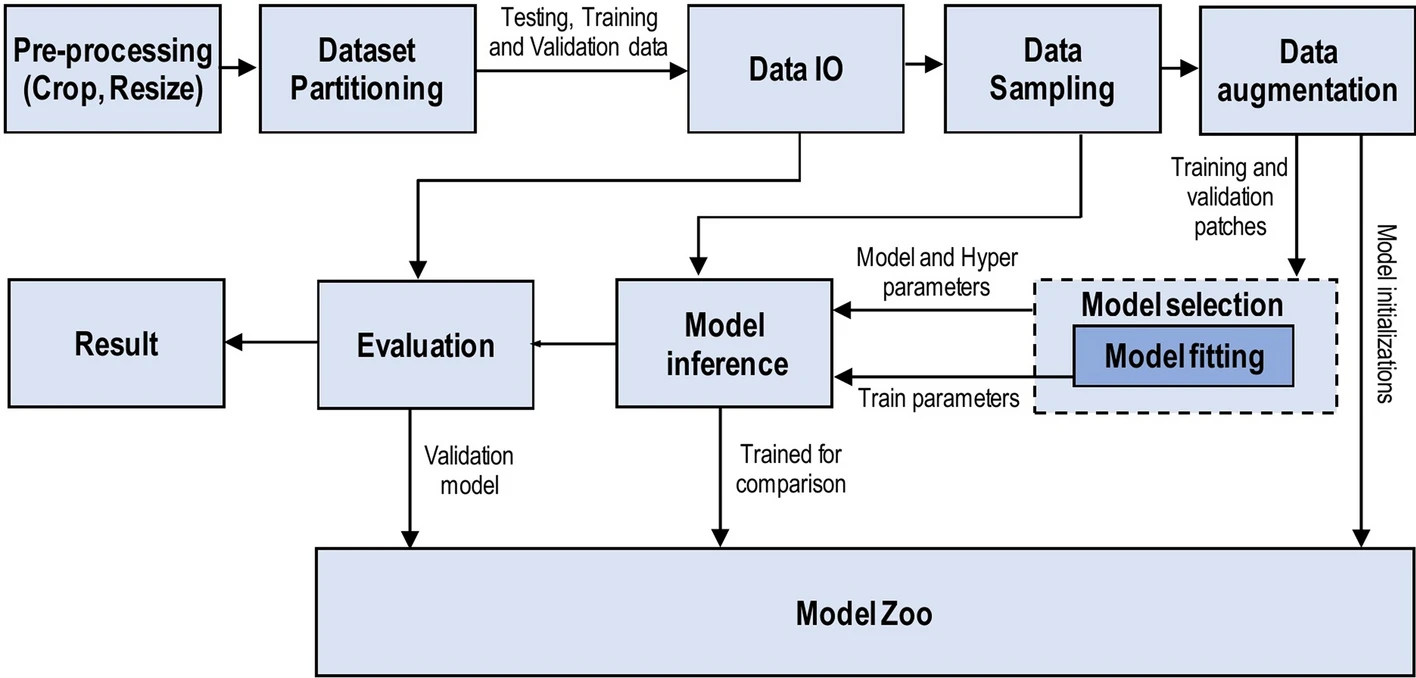
\includegraphics[scale=0.26]{./figures/Pipeline.png}
	\caption{Generic deep learning pipeline as outlined by\citeauthor{alzubaidi2021review}}~\label{fig:pipeline}
\end{figure}

\subsubsection{Normalisation of the data}
When working with pre-trained models, normalisation is commonly carried out to adjust for the distribution of the dataset that the model was originally trained on. This can be paired with cropping and resizing the images of the given dataset to fit the dimensions required as input to the pre-trained model. Such normalisation can be related to the first step in the pipeline proposed by Alzubaidini et al., namely  ``Pre-processing (Crop, Resize)'' in Figure~\ref{fig:pipeline}. The normalisation statistics for pre-trained models loaded via PyTorch are generally given as is the case for AlexNet\citep{pytorchAlexNet}. As an implicit hypothesis, the normalisation of the data according to the model that's employed should enable a frictionless usage of said model.


\subsubsection{Balancing of the Dataset}\label{balancingtheory}
As~\citeauthor{kaurbalancing} elucidate in their Systematic Review on Imbalanced Data Challenges
in Machine Learning, an imbalanced dataset can lead to classifications being skewed in favour of the majority class. When working with multi-class classification problems, this applies to the classes with clearly more data points than the other classes. While measures like the Imbalanced Ratio \citep{kulkarni2020foundations} do exist to quantify how unbalanced a dataset is, there commonly doesn't appear to be a strict cut-off value for when a dataset is deemed ``unbalanced''. Nonetheless, it's evident that unbalanced datasets must be dealt with, as Kaur et al\@. describe how the accuracy in these favour the majority class, yielding potentially better accuracy for the majority class while yielding lower accuracy for the minority class.~\citeauthor{kaurbalancing} also present various methods which essentially rely on oversampling or undersampling classes, sometimes according to some measure \citep{kulkarni2020foundations}. In the generic pipeline for deep learning by Alzubaido et al., Data Sampling can also be found in the early stages of the proposed pipeline, see Figure~\ref{fig:pipeline} PyTorch provides various samplers, among them~\cite{pytorchTorchutilsdatax2014}, which allows to sample elements according to some given probabilities. In order to balance out a dataset using WeightedRandomSampler provided by PyTorch, the probabilities with which data from a class is drawn needs to be calculated. The code implementing the WeightedRandomSampler is provided in the appendix, see~\ref{weightedsampler}. These probabilities can be determined by dividing 1 by the number of samples in a class. Following this theoretical foundation, the hypothesis is that a balancing of the data improves accuracy as compared to a model which learned on unbalanced data.

\subsubsection{Data Augmentation}\label{augmentationtheory}
Small data size and lack of variation in the data is associated with false predictions and worse accuracy by~\citeauthor{maharana2022review}. Data quality issues plague many areas of Machine Learning.~\citeauthor{maharana2022review} note that by means of data augmentation, more data can be generated from limited amounts of data and there's also the potential to combat overfitting. Data augmentation is commonly assigned to the data preprocessing part of the deep learning pipeline. Common data augmentation techniques listed by Maharana include: flipping, rotation, noise, shifting, cropping, PCA jittering GAN, and WGAN\@. All these methods listed could, in theory, increase variation in the data and thus avoid overfitting, producing a model more capable of generalisation and capturing a plethora of features instead of being limited to a smaller pool of features of an unaugmented dataset. Considering this, the hypothesis that arises is that data augmentation will help with overall accuracy and overfitting, possibly leading to less false positives and more true positives across for instance a confusion matrix\@.

\subsubsection{Batch Normalisation}\label{batchnormtheory}
\citeauthor{santurkar2018does} describe how for Batch Normalisation additional layers are added to the architecture of the network which set the mean and variance of the output to zero and one respectively \citep{santurkar2018does}. In order to retain model expressivity the batch normalised inputs are also shifted and scaled based on trainable parameters. The idea of the Internal Covariate Shift is described by Santurkar et al\@. as one of the reasons batch normalisation was invented. Internal Covariate Shift, it is speculated, essentially is a change of the distribution of inputs to a layer in the network caused by an update of parameters to the previous layers. Furthermore, Internal Covariate Shift is hence presumed to have as a consequence a constant shift of the underlying training problem. However, this remains a controversial concept, as Santurkar et al\@. actually argue that batch normalisation does not reduce Internal Covariate Shift at all. The authors identify the key effect of batch normalisation to be the reparametrisation of the underlying optimisation problem in order to make it more stable. Despite presumably not dealing with the Internal Covariate Shift, batch normalisation thus potentially is a useful addition to a deep learning architecture. Extrapolating from that one arrives at the hypothesis that a network with batch normalisation performs better across given metrics as compared to a network without batch normalisation, ceteris paribus.


\subsubsection{Evaluation Metrics}
Hand et al\@. define various evaluation metrics~\citep{hand2021f} which are commonly found throughout the literature. To facilitate legibility, the following abbreviations are used: total number of positives (P), total number of negatives (N), true positives (TP), true negatives (TN), false positives (FP) and false negatives (FN). A quick definition of these metrics shall be given here as proposed by~\cite{hand2021f}. 

\begin{center}
	Accuracy = $\frac{TP + TN}{P + N}$ \hspace{4em} Precision = $\frac{TP}{TP + FP}$ \hspace{4em} Recall = $\frac{TP}{TP + FN}$ \newline
\end{center}
\begin{center}
	F1-Score = $2 \cdot \frac{Precision \cdot Recall}{Precision + Recall}$
\end{center}
\subsection{Model Architectures}\label{architectures}

\subsubsection{SimpleCNN}\label{simplecnn}

Our SimpleCNN model, designed as an initial exploration of deep learning, contains two primary convolutional layers. The choice of this architecture was motivated by the goal of understanding the basic mechanisms of neural networks in processing and classifying image data. The model uses LeakyReLU activation to avoid the vanishing gradient problem and to ensure effective backpropagation even at small gradient values. The first convolution layer uses 32 filters with a kernel size of 5$\times$5, a stride of 1 and `equal' padding, which preserves the dimension of the input images. This is followed by a max-pooling layer with a kernel size of 2, which aims to reduce the spatial dimensions while keeping the important features to optimize the model's ability to detect significant patterns without considerable data loss. Subsequently, a second convolution sequence increases the depth to 64 filters, improving the model's ability to extract more complex features. This setup is again followed by LeakyReLU activation and max-pooling, further refining the feature extraction process. The architecture concludes with a linear layer that maps the high-level features to the output classes, with a softmax function to interpret the outputs as class probabilities.

As our project progressed and our understanding deepened, we enhanced the initial SimpleCNN model by introducing an additional convolutional layer and incorporating batch normalization and dropout techniques, aiming for improved accuracy and generalization. The modified SimpleCNN architecture begins with a convolutional layer designed for single-channel (grayscale) images to match the format of the MNIST dataset. This layer, consisting of 32 filters with a kernel size of 3$\times$3 and `same' padding, is followed by batch normalization and ReLU activation, which promotes nonlinearity while maintaining normalization across the inputs of the network. A dropout rate of 0.25 after max pooling aims to mitigate overfitting by randomly omitting a portion of the features during the training process. As the model progresses, the second and third convolutional layers increase the filter count to 64 and then 128, respectively, each augmented with batch normalization, ReLU activation, max pooling, and a consistent dropout rate of 0.25. This architectural depth ensures the extraction of increasingly complex features essential for recognizing diverse patterns in handwritten digits. The concluding segment of the model comprises a fully connected layer transitioning from the convolutional output to 256 units, followed by batch normalization and a higher dropout rate of 0.5, further combating overfitting. The final linear layer maps these processed features to the ten class outputs corresponding to the MNIST dataset's digit categories.

The transition from the SimpleCNN model, which was tailored for the MNIST dataset, to the model customized for the PathMNIST challenge required some adjustments to account the different characteristics of the two datasets. The most important change was to adapt the input layer to include 3-channel RGB images for PathMNIST, as opposed to the single-channel configuration developed for MNIST's grayscale images. This change is important to take advantage of the color information that is critical in medical imaging for identifying different tissue types. Despite this adaptation, the core architecture~-~consisting of convolutional layers, batch normalization, ReLU activation, and dropout layers~-~remained consistent between models.

For a detailed implementation of all versions of the model, refer to the Appendix Section~\ref{codeSnippets}.\@
\subsubsection{ResNet}\label{resnet}
The Residual Network architecture (ResNet) was first introduced by \citep{he2015deep} in their paper "Deep Residual Learning for Image Recognition". This marked a big advancement in deep learning for computer vision, as previous model architectures did not have the ability to effectively scale with more layers. These models would, among other issues, run into a vanishing or exploding gradient problem, making deeper layers less usefull and impacting performance. To combat this, ResNet introduces a solution using residual blocks, as shown in Figure \ref{fig:residualBlock}. The input X goes through two paths. One is called a skip connection and carries the original input to a junction point. The other carries the input through multiple convolutional layers to process it. Following the first layer, the input is passed through a ReLu function, introducing non-linearity to the model. Then it is passed trough a second convolutional layer, which returns a residual function. In the end, the learned residual function is added to the original input.
\begin{figure}[ht]
    \centering
    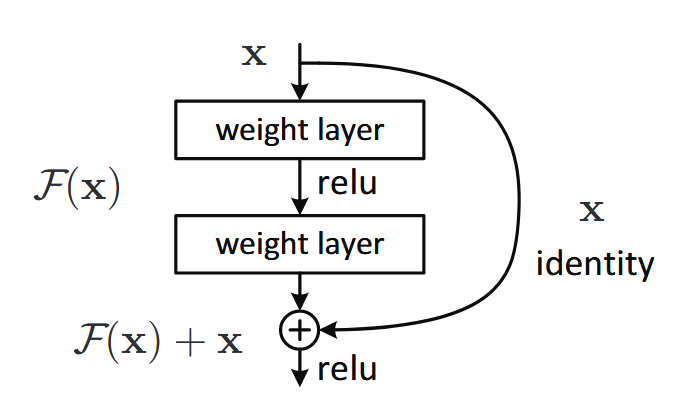
\includegraphics[width=0.7\textwidth]{figures/ResidualBlock.png}
    \caption{Residual Block as outlined by \citeauthor{he2015deep}.}\label{fig:residualBlock}
\end{figure}

\subsubsubsection{ResNet18 and ResNet32:}\label{resnet18}
Using the block shown in Figure \ref{fig:residualBlock}, the researchers built two networks, that are now commonly used. ResNet18, containing 18 and ResNet32, containing 32 layers, made of these two-layer residual blocks. These networks are designed for simpler tasks and limited training resources. They offer great performance relative to their size.

\begin{figure}[ht]
    \centering
    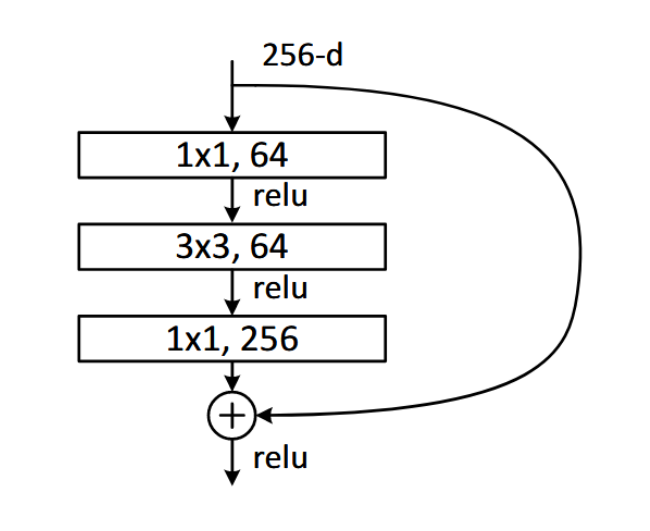
\includegraphics[width=0.6\textwidth]{figures/BottleNeckBlock.png}
    \caption{Bottleneck Block as outlined by \citeauthor{he2015deep}.}\label{fig:bottleneckBlock}
\end{figure}

\subsubsubsection{ResNet50, ResNet101 and ResNet152:}\label{resnet152}
In order to further upscale this technology, the researchers introduced a modification to the two-layer structure. As seen in Figure \ref{fig:bottleneckBlock}, the researchers created a bottleneck block. This block features two convolutional layers with a 1$\times$1 convolution and a middle layer with a  3$\times$3 convolution. The first layer down scales the input, which is then forwarded to the next layer with a 3$\times$3 convolution. This middle layer is the core of the bottleneck block, where the actual feature extraction happens. Then the third layer upscales the input back to its original size and returns the output for the block. These Models work well for large and complicated datasets but are more computationally demanding than their two-layer counterparts. 
\subsubsection{Xception}\label{xception}

To understand the Xception model, one must become familiar with depth-separable convolutions. This technique is a convolution operation that divides into two different stages to increase computational efficiency. Initially, a depth-wise convolution applies a single filter to each input channel. Subsequently, a point-wise convolution~-~characterized by a 1$\times$1 kernel~-~combines the outputs from the depth-wise step across the channels. This factorization significantly reduces the number of parameters and calculations and enables more efficient training. Batch normalization follows each convolution and promotes stable learning by normalizing the ReLU activations of the layer.

As seen in Figure~\ref{fig:xceptionArchitecture} the architecture of Xception, as detailed by \citep{chollet2017xception}, is structured into three primary flows. The entry flow prepares the network with initial convolutions and pooling to create condensed feature maps from the input images. It starts with two standard convolutions, followed by a series of separable convolutions that increase the depth while compressing spatial dimensions. This is achieved using a combination of 1$\times$1 convolutions for channel-wise feature processing and 3$\times$3 convolutions for capturing spatial information, each followed by max pooling to halve the feature map dimensions progressively. This step reduces the initial input image size from 299$\times$299$\times$3 to 19$\times$19$\times$728. Central to Xception's design is the middle flow, which repeatedly applies depthwise separable convolutions to process and refine the features. This part of the network is designed to be repeated eight times, allowing the model to learn increasingly complex patterns without affecting the dimensions. The exit flow then expands the feature maps through additional separable convolutions, incorporating a mix of channel-wise and spatial feature extraction before concluding with global average pooling. This step reduces each map to a single vector, capturing the essence of the input data in a form suitable for classification. The network concludes with a logistic regression layer, such as softmax, to output the final class probabilities.

\begin{figure}[ht]
    \centering
    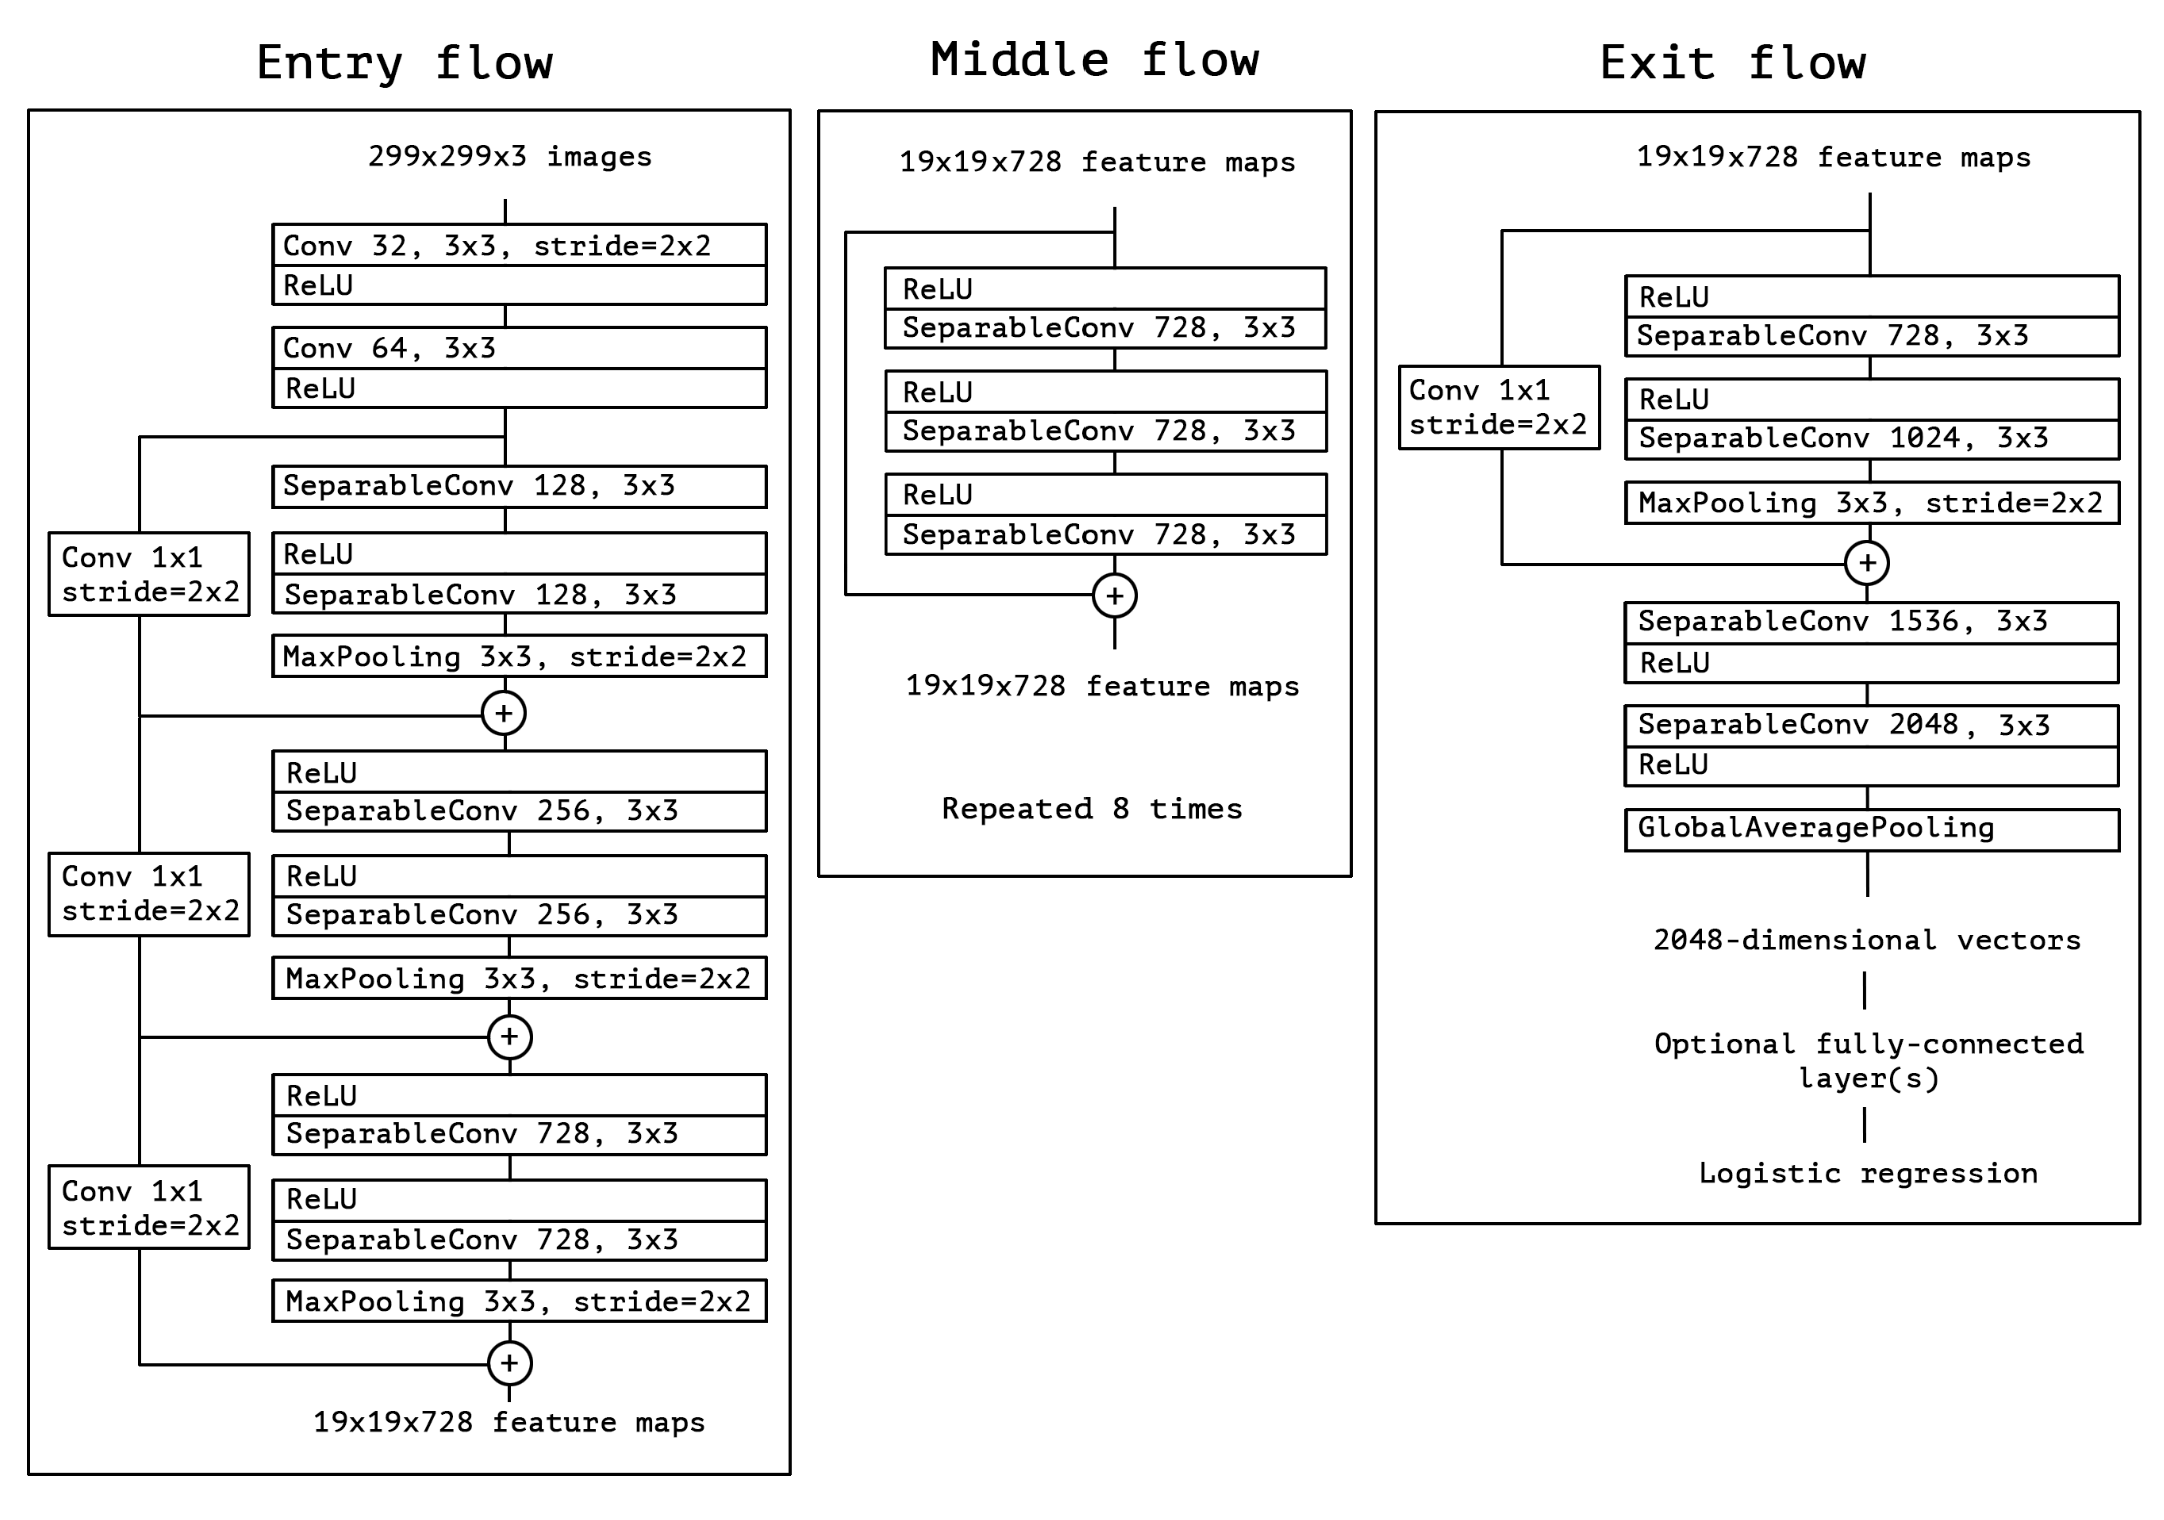
\includegraphics[width=0.9\textwidth]{figures/xception_architecture.png}
    \caption{Xceptions architecture as outlined by \citeauthor{chollet2017xception}.}\label{fig:xceptionArchitecture}
\end{figure}
\section{Discussion}\label{discussion}

\subsubsubsection{ResNet:}\label{ResNetDiscussion}
During the training we observed a slight but consistent difference between the validation accuracy after training and the final accuracy on our unlabeled dataset for Kaggle. One idea is, that the dataset used for our submission has more instances of the problematic classes our models struggled with. Over all we managed to improve the performance of our models by a lot, when compared to our first attempts. For the future we should put bigger focus on reproducibility and consistency when doing multiple training runs to test differences between hyperparameters. Our choice of optimizer here, while delivering good results, might have been just a statistical anomaly during testing and it would have made sense to do more in-depth testing on different optimizers. One other approach that might be worth looking in to is to minimize the non-deterministic behaviour duric training with cuda. One way would be to set CuDNN in PyTorch to deterministic mode. Here it would be interesting to see how much of an performance impact this has on the training. We also observed that deeper models would take many more epochs than smaller models until they converged. Some instances of ResNet152 trained for 80 epochs, before early stopping was triggered. Here, the question could be raised how important the gained improvement is, compared to smaller models. It would also be interesting to see how these performance differences would change with larger datasets. Another path that we would like to look into more are ensemble methods. A different implementation, or just the combination of more models of different architectures with our current approach might lead to even better results. 
\section{Conclusion}\label{conclusion}
//TODO


\begin{figure}
  \centering
  \fbox{\rule[-.5cm]{0cm}{4cm} \rule[-.5cm]{4cm}{0cm}}
  \caption{Sample figure caption.}
\end{figure}

\begin{table}
  \caption{Sample table title}
  \label{sample-table}
  \centering
  \begin{tabular}{lll}
    \toprule
    \multicolumn{2}{c}{Part}                   \\
    \cmidrule(r){1-2}
    Name     & Description     & Size ($\mu$m) \\
    \midrule
    Dendrite & Input terminal  & $\sim$100     \\
    Axon     & Output terminal & $\sim$10      \\
    Soma     & Cell body       & up to $10^6$  \\
    \bottomrule
  \end{tabular}
\end{table}

% \begin{ack}
% Use unnumbered first level headings for the acknowledgments. All acknowledgments
% go at the end of the paper before the list of references. Moreover, you are required to declare
% funding (financial activities supporting the submitted work) and competing interests (related financial activities outside the submitted work).
% More information about this disclosure can be found at: \url{https://neurips.cc/Conferences/2022/PaperInformation/FundingDisclosure}.


% Do {\bf not} include this section in the anonymized submission, only in the final paper. You can use the \texttt{ack} environment provided in the style file to autmoatically hide this section in the anonymized submission.
% \end{ack}

%#\section{Notation}
%% SOURCE: https://github.com/goodfeli/dlbook_notation/blob/master/math_commands.tex
% Quote from github "We make them freely available for anyone to use."


% Sometimes we have to include the following line to get this section
% included in the Table of Contents despite being a chapter*
This section provides a concise reference describing notation as used in the book by \citet{goodfellow2016deep}.
If you are unfamiliar with any of the corresponding mathematical concepts,
\citet{goodfellow2016deep} describe most of these ideas in
chapters 2--4. \\[0.7cm]

% Need to use minipage to keep title of table on same page as table
% This is a hack to put a little title over the table
% We cannot use "\section*", etc., they appear in the table of contents.
% tocdepth does not work on this chapter.
\centerline{\bf Numbers and Arrays}
\bgroup
% The \arraystretch definition here increases the space between rows in the table,
% so that \displaystyle math has more vertical space.
\def\arraystretch{1.5}
\begin{tabular}{cp{3.25in}}
$\displaystyle a$ & A scalar (integer or real)\\
$\displaystyle \va$ & A vector\\
$\displaystyle \mA$ & A matrix\\
$\displaystyle \tA$ & A tensor\\
$\displaystyle \mI_n$ & Identity matrix with $n$ rows and $n$ columns\\
$\displaystyle \mI$ & Identity matrix with dimensionality implied by context\\
$\displaystyle \ve^{(i)}$ & Standard basis vector $[0,\dots,0,1,0,\dots,0]$ with a 1 at position $i$\\
$\displaystyle \text{diag}(\va)$ & A square, diagonal matrix with diagonal entries given by $\va$\\
$\displaystyle \ra$ & A scalar random variable\\
$\displaystyle \rva$ & A vector-valued random variable\\
$\displaystyle \rmA$ & A matrix-valued random variable\\
\end{tabular}

\vspace{0.5cm}
\centerline{\bf Sets and Graphs}
\bgroup
\def\arraystretch{1.5}
\begin{tabular}{cp{3.25in}}
$\displaystyle \sA$ & A set\\
$\displaystyle \R$ & The set of real numbers \\
% NOTE: do not use \R^+, because it is ambiguous whether:
% - It includes 0
% - It includes only real numbers, or also infinity.
% We usually do not include infinity, so we may explicitly write
% [0, \infty) to include 0
% (0, \infty) to not include 0
$\displaystyle \{0, 1\}$ & The set containing 0 and 1 \\
$\displaystyle \{0, 1, \dots, n \}$ & The set of all integers between $0$ and $n$\\
$\displaystyle [a, b]$ & The real interval including $a$ and $b$\\
$\displaystyle (a, b]$ & The real interval excluding $a$ but including $b$\\
$\displaystyle \sA \backslash \sB$ & Set subtraction, i.e., the set containing the elements of $\sA$ that are not in $\sB$\\
$\displaystyle \gG$ & A graph\\
$\displaystyle \parents_\gG(\ervx_i)$ & The parents of $\ervx_i$ in $\gG$
\end{tabular}

\vspace{0.5cm}
\centerline{\bf Indexing}
\bgroup
\def\arraystretch{1.5}
\begin{tabular}{cp{3.25in}}
$\displaystyle \eva_i$ & Element $i$ of vector $\va$, with indexing starting at 1 \\
$\displaystyle \eva_{-i}$ & All elements of vector $\va$ except for element $i$ \\
$\displaystyle \emA_{i,j}$ & Element $i, j$ of matrix $\mA$ \\
$\displaystyle \mA_{i, :}$ & Row $i$ of matrix $\mA$ \\
$\displaystyle \mA_{:, i}$ & Column $i$ of matrix $\mA$ \\
$\displaystyle \etA_{i, j, k}$ & Element $(i, j, k)$ of a 3-D tensor $\tA$\\
$\displaystyle \tA_{:, :, i}$ & 2-D slice of a 3-D tensor\\
$\displaystyle \erva_i$ & Element $i$ of the random vector $\rva$ \\
\end{tabular}

\vspace{0.5cm}
\centerline{\bf Linear Algebra Operations}
\bgroup
\def\arraystretch{1.5}
\begin{tabular}{cp{3.25in}}
$\displaystyle \mA^\top$ & Transpose of matrix $\mA$ \\
$\displaystyle \mA^+$ & Moore-Penrose pseudoinverse of $\mA$\\
$\displaystyle \mA \odot \mB $ & Element-wise (Hadamard) product of $\mA$ and $\mB$ \\
% Wikipedia uses \circ for element-wise multiplication but this could be confused with function composition
$\displaystyle \mathrm{det}(\mA)$ & Determinant of $\mA$ \\
\end{tabular}

\vspace{0.5cm}
\centerline{\bf Calculus}
\bgroup
\def\arraystretch{1.5}
\begin{tabular}{cp{3.25in}}
% NOTE: the [2ex] on the next line adds extra height to that row of the table.
% Without that command, the fraction on the first line is too tall and collides
% with the fraction on the second line.
$\displaystyle\frac{d y} {d x}$ & Derivative of $y$ with respect to $x$\\ [2ex]
$\displaystyle \frac{\partial y} {\partial x} $ & Partial derivative of $y$ with respect to $x$ \\
$\displaystyle \nabla_\vx y $ & Gradient of $y$ with respect to $\vx$ \\
$\displaystyle \nabla_\mX y $ & Matrix derivatives of $y$ with respect to $\mX$ \\
$\displaystyle \nabla_\tX y $ & Tensor containing derivatives of $y$ with respect to $\tX$ \\
$\displaystyle \frac{\partial f}{\partial \vx} $ & Jacobian matrix $\mJ \in \R^{m\times n}$ of $f: \R^n \rightarrow \R^m$\\
$\displaystyle \nabla_\vx^2 f(\vx)\text{ or }\mH( f)(\vx)$ & The Hessian matrix of $f$ at input point $\vx$\\
$\displaystyle \int f(\vx) d\vx $ & Definite integral over the entire domain of $\vx$ \\
$\displaystyle \int_\sS f(\vx) d\vx$ & Definite integral with respect to $\vx$ over the set $\sS$ \\
\end{tabular}

\vspace{0.5cm}
\centerline{\bf Probability and Information Theory}
\bgroup
\def\arraystretch{1.5}
\begin{tabular}{cp{3.25in}}
$\displaystyle \ra \bot \rb$ & The random variables $\ra$ and $\rb$ are independent\\
$\displaystyle \ra \bot \rb \mid \rc $ & They are conditionally independent given $\rc$\\
$\displaystyle P(\ra)$ & A probability distribution over a discrete variable\\
$\displaystyle p(\ra)$ & A probability distribution over a continuous variable, or over
a variable whose type has not been specified\\
$\displaystyle \ra \sim P$ & Random variable $\ra$ has distribution $P$\\% so thing on left of \sim should always be a random variable, with name beginning with \r
$\displaystyle  \E_{\rx\sim P} [ f(x) ]\text{ or } \E f(x)$ & Expectation of $f(x)$ with respect to $P(\rx)$ \\
$\displaystyle \Var(f(x)) $ &  Variance of $f(x)$ under $P(\rx)$ \\
$\displaystyle \Cov(f(x),g(x)) $ & Covariance of $f(x)$ and $g(x)$ under $P(\rx)$\\
$\displaystyle H(\rx) $ & Shannon entropy of the random variable $\rx$\\
$\displaystyle \KL ( P \Vert Q ) $ & Kullback-Leibler divergence of P and Q \\
$\displaystyle \mathcal{N} ( \vx ; \vmu , \mSigma)$ & Gaussian distribution %
over $\vx$ with mean $\vmu$ and covariance $\mSigma$ \\
\end{tabular}

\vspace{0.5cm}
\centerline{\bf Functions}
\bgroup
\def\arraystretch{1.5}
\begin{tabular}{cp{3.25in}}
$\displaystyle f: \sA \rightarrow \sB$ & The function $f$ with domain $\sA$ and range $\sB$\\
$\displaystyle f \circ g $ & Composition of the functions $f$ and $g$ \\
  $\displaystyle f(\vx ; \vtheta) $ & A function of $\vx$ parametrized by $\vtheta$.
  (Sometimes we write $f(\vx)$ and omit the argument $\vtheta$ to lighten notation) \\
$\displaystyle \log x$ & Natural logarithm of $x$ \\
$\displaystyle \sigma(x)$ & Logistic sigmoid, $\displaystyle \frac{1} {1 + \exp(-x)}$ \\
$\displaystyle \zeta(x)$ & Softplus, $\log(1 + \exp(x))$ \\
$\displaystyle || \vx ||_p $ & $\normlp$ norm of $\vx$ \\
$\displaystyle || \vx || $ & $\normltwo$ norm of $\vx$ \\
$\displaystyle x^+$ & Positive part of $x$, i.e., $\max(0,x)$\\
$\displaystyle \1_\mathrm{condition}$ & is 1 if the condition is true, 0 otherwise\\
\end{tabular}

Sometimes we use a function $f$ whose argument is a scalar but apply
it to a vector, matrix, or tensor: $f(\vx)$, $f(\mX)$, or $f(\tX)$.
This denotes the application of $f$ to the
array element-wise. For example, if $\tC = \sigma(\tX)$, then $\etC_{i,j,k} = \sigma(\etX_{i,j,k})$
for all valid values of $i$, $j$ and $k$.

\vspace{0.5cm}
\centerline{\bf Datasets and Distributions}
\bgroup
\def\arraystretch{1.5}
\begin{tabular}{cp{3.25in}}
$\displaystyle \pdata$ & The data generating distribution\\
$\displaystyle \ptrain$ & The empirical distribution defined by the training set\\
$\displaystyle \sX$ & A set of training examples\\
$\displaystyle \vx^{(i)}$ & The $i$-th example (input) from a dataset\\
$\displaystyle y^{(i)}\text{ or }\vy^{(i)}$ & The target associated with $\vx^{(i)}$ for supervised learning\\
$\displaystyle \mX$ & The $m \times n$ matrix with input example $\vx^{(i)}$ in row $\mX_{i,:}$\\
\end{tabular}

\clearpage



\bibliography{bibliography}
\bibliographystyle{abbrvnat}


%%%%%%%%%%%%%%%%%%%%%%%%%%%%%%%%%%%%%%%%%%%%%%%%%%%%%%%%%%%%%%%%%%%%%%%%%%%%%%%%%%%%%%%%%%%%%%%%%%%%
%% Declaration of Authorship
%%%%%%%%%%%%%%%%%%%%%%%%%%%%%%%%%%%%%%%%%%%%%%%%%%%%%%%%%%%%%%%%%%%%%%%%%%%%%%%%%%%%%%%%%%%%%%%%%%%%


\newpage
{\parindent 0cm
%%%%%%%%%%%%%%%%%%%%%%%%%%German%%%%%%%%%%%%%%%%%%%%%%%%%%%%%%
\section*{Declaration of Authorship}
Ich erkläre hiermit gemäß § 9 Abs. 12 APO, dass ich die vorstehende Projektarbeit selbstständig verfasst und keine anderen als die angegebenen Quellen und Hilfsmittel benutzt habe. Des Weiteren erkläre ich, dass die digitale Fassung der gedruckten Ausfertigung der Projektarbeit ausnahmslos in Inhalt und Wortlaut entspricht und zur Kenntnis genommen wurde, dass diese digitale Fassung einer durch Software unterstützten, anonymisierten Prüfung auf Plagiate unterzogen werden kann.\\
\vspace{2\baselineskip}
  
Bamberg, \today

\rule[0.5em]{14em}{0.5pt} \hspace{0.25\linewidth}\rule[0.5em]{14em}{0.5pt}
\vspace{1em}
\hspace{4em} (Place, Date) \hspace{0.51\linewidth} (Signature)

Bamberg, \today

\rule[0.5em]{14em}{0.5pt} \hspace{0.25\linewidth}\rule[0.5em]{14em}{0.5pt}
\vspace{1em}
\hspace{4em} (Place, Date) \hspace{0.51\linewidth} (Signature)

Bamberg, \today

\rule[0.5em]{14em}{0.5pt} \hspace{0.25\linewidth}\rule[0.5em]{14em}{0.5pt}
\vspace{1em}
\hspace{4em} (Place, Date) \hspace{0.51\linewidth} (Signature)
}



%%%%%%%%%%%%%%%%%%%%%%%%%%%%%%%%%%%%%%%%%%%%%%%%%%%%%%%%%%%%


%%%%%%%%%%%%%%%%%%%%%%%%%%%%%%%%%%%%%%%%%%%%%%%%%%%%%%%%%%%%

\newpage
\appendix
\section{Appendix}
\subsection{SimpleCNN architecture}\label{codeSnippets}
Initial version of our SimpleCNN, including two convulutional layers:\@

\begin{minted}[mathescape, linenos, fontsize=\scriptsize]{python}
class SimpleCNN(nn.Module):
    def __init__(self, num_classes=10):
        super(SimpleCNN, self).__init__()
        self.conv1 = nn.Sequential(
            nn.Conv2d(
                in_channels = 1,
                out_channels = 32,
                kernel_size = 3,
                stride=1,
                padding="same"
            ),
            nn.LeakyReLU(),
            nn.MaxPool2d(kernel_size=2),
        )
        self.conv2 = nn.Sequential(
            nn.Conv2d(32,64,3,1,"same"),
            nn.LeakyReLU(),
            nn.MaxPool2d(kernel_size=2),
        )
        self.out = nn.Linear(64*7*7, num_classes)

     def forward(self, x):
        x = self.conv1(x)
        x = self.conv2(x)
        x = x.view(-1, 64*7*7)
        output = self.out()
        return torch.log_softmax(output, dim=1)
\end{minted}


Structure of the improved version of the SimpleCNN using three convolutional layers, Batch normalization and Dropout:\@

\begin{minted}[mathescape, linenos, fontsize=\scriptsize]{python}
class SimpleCNN(nn.Module):
    def __init__(self, num_classes=10):
        super(SimpleCNN, self).__init__()
        self.conv1 = nn.Sequential(
            nn.Conv2d(1, 32, kernel_size=3, stride=1, padding="same"),
            nn.BatchNorm2d(32),
            nn.ReLU(),
            nn.MaxPool2d(kernel_size=2),
            nn.Dropout(0.25)
        )
        self.conv2 = nn.Sequential(
            nn.Conv2d(32, 64, kernel_size=3, stride=1, padding="same"),
            nn.BatchNorm2d(64),
            nn.ReLU(),
            nn.MaxPool2d(2),
            nn.Dropout(0.25)
        )
        self.conv3 = nn.Sequential(
            nn.Conv2d(64, 128, kernel_size=3, stride=1, padding="same"),
            nn.BatchNorm2d(128),
            nn.ReLU(),
            nn.MaxPool2d(2),
            nn.Dropout(0.25)
        )
        self.fc1 = nn.Linear(128 * 3 * 3, 256)
        self.fc_bn = nn.BatchNorm1d(256)
        self.dropout_fc = nn.Dropout(0.5)
        self.fc2 = nn.Linear(256, num_classes)

    def forward(self, x):
        x = self.conv1(x)
        x = self.conv2(x)
        x = self.conv3(x)
        x = x.view(-1, 128 * 3 * 3)
        x = F.relu(self.fc_bn(self.fc1(x)))
        x = self.dropout_fc(x)
        x = self.fc2(x)
        return torch.log_softmax(x, dim=1)
\end{minted}
    

Structure of the improved version of the SimpleCNN for the PathMNIST dataset:\@

\begin{minted}[mathescape, linenos, fontsize=\scriptsize]{python}
class SimpleCNN(nn.Module):
    def __init__(self, num_classes=10):
        super(SimpleCNN, self).__init__()
        self.conv1 = nn.Sequential(
            nn.Conv2d(3, 32, kernel_size=3, stride=1, padding="same"),
            nn.BatchNorm2d(32),
            nn.ReLU(),
            nn.MaxPool2d(kernel_size=2),
            nn.Dropout(0.25)
        )
        self.conv2 = nn.Sequential(
            nn.Conv2d(32, 64, kernel_size=3, stride=1, padding="same"),
            nn.BatchNorm2d(64),
            nn.ReLU(),
            nn.MaxPool2d(2),
            nn.Dropout(0.25)
        )
        self.conv3 = nn.Sequential(
            nn.Conv2d(64, 128, kernel_size=3, stride=1, padding="same"),
            nn.BatchNorm2d(128),
            nn.ReLU(),
            nn.MaxPool2d(2),
            nn.Dropout(0.25)
        )
        self.fc1 = nn.Linear(128 * 3 * 3, 256)
        self.fc_bn = nn.BatchNorm1d(256)
        self.dropout_fc = nn.Dropout(0.5)
        self.fc2 = nn.Linear(256, num_classes)

    def forward(self, x):
        x = self.conv1(x)
        x = self.conv2(x)
        x = self.conv3(x)
        x = x.view(-1, 128 * 3 * 3)
        x = F.relu(self.fc_bn(self.fc1(x)))
        x = self.dropout_fc(x)
        x = self.fc2(x)
        return torch.log_softmax(x, dim=1)
\end{minted}


\end{document}
